
% This LaTeX was auto-generated from MATLAB code.
% To make changes, update the MATLAB code and republish this document.

\documentclass[12pt]{article}
%%% ========== Package setup ==========
\usepackage{listings}   % Script listing package
\usepackage{wrapfig}    % Wrap Figure or table package
\usepackage{multicol}   % Multicolumn package
\usepackage{pdfpages}   % Include pdf files

%%% ========== Format setup ==========
%% Setup chinese words encoder
\usepackage{xeCJK}
\XeTeXlinebreaklocale "zh"
\XeTeXlinebreakskip = 0pt plus 1pt

%% More word fonts
\usepackage{fontspec}
\setmainfont{Times New Roman}
\renewcommand{\familydefault}{\rmdefault}
\setCJKmainfont{標楷體}

%% Chinese paragraph format
\usepackage{indentfirst}
\setlength{\parindent}{2em}

%% Page margin
\usepackage[a4paper, total={6in,8in}]{geometry}

%%% ========== Document ==========

\sloppy
\definecolor{lightgray}{gray}{0.5}
\setlength{\parindent}{0pt}

\begin{document}

\pagenumbering{gobble}
\newcommand{\MakeTitlePage}[1]{
\begin{titlepage}
    \begin{center}

        \fontsize{50}{10}
        \selectfont
        Linear Systems

        \vspace{1cm}

        \fontsize{30}{10}
        \selectfont
        Final exam

        \vspace{11cm}

        \begin{tabular}{ r l }
            班級: & 航太四A \\ [10pt]
            姓名: & 吳柏勳 \\ [10pt]
            學號: & 407430635 \\ [10pt]
            座號: & 4 \\ [10pt]
        \end{tabular}

    \end{center}
\end{titlepage}
}
\MakeTitlePage{3}
\includepdf[pages=1-4]{handout.pdf}

\subsection*{\#4}

\begin{verbatim}
clear;clc;close all
% global V alpha gamma lambda

% Setup parameters
g = 9.81;               % gravity(m/s^2)
m = 95000;              % mass(kg)
S = 153;                % wing area(m^2)
rho = 0.7782;           % air density(kg/m^2)
epsilon = 3;            % angle between thrust and fuselage(deg)
T = 60000;              % thrust(N)
C_L0 = 0;               % (1)
C_D0 = 0.07351;         % (1)
C_La = 0.1;             % (1/deg)
C_Da = 0.05;            % (1/deg)

% Setup unknown variables
syms alpha              % angle of attack(deg)
syms gamma              % flight path angle(deg)
syms V                  % velocity(m/s)

% Calculate aerodynamic parameters
C_L = C_L0 + C_La*alpha;
C_D = C_D0 + C_Da*alpha;
L = 0.5*rho*(V*cosd(alpha))^2*S*C_L;
D = 0.5*rho*(V*cosd(alpha))^2*S*C_D;

% Calculate force vectors in body fix coordinate([et; en])
Thrust = T*[cosd(alpha+epsilon); sind(alpha+epsilon)];
Weight = m*g*[-sind(gamma); -cosd(gamma)];
Lift = L*[0; 1];
Drag = D*[-1; 0];
Acceleration = [0; 0];

% Create equation of motion(EOM) and rate of climb(RC)
EOM = Thrust + Weight + Lift + Drag - m*Acceleration;
RC = V*sind(gamma);

% Setup the minimize equation and Hamiltonian
syms lambda1 lambda2
L = -RC;
lambda = [lambda1; lambda2];
f = EOM;
H = L + lambda'*f;

% Setup the necessary condition and constrain equation
dH = [diff(H, V); diff(H, alpha); diff(H, gamma)];
sym_eqns = [dH; f];

% Setup the solver option
opt = optimoptions('fsolve', 'Display', 'none', 'OutputFcn', @outputfun);

% Setup the equation function and initial condition
fun_eqn = @(x) double(subs(sym_eqns, [V alpha gamma lambda1 lambda2], x));
x0 = [100 20 20 0 0];

% Using "fsolve" to figure out the nonlinear equations
sol = fsolve(fun_eqn, x0, opt);
max_RC = sol(1)*sind(sol(3))
\end{verbatim}


\color{lightgray} \begin{verbatim}
    max_RC =

      -30.7666

    \end{verbatim} \color{black}

    \begin{figure}
            \centering

            \includegraphics [width=2.9in]{HW3_01.eps}
            \caption{Velocity}
            \vspace{10pt}

            \includegraphics [width=2.9in]{HW3_02.eps}
            \caption{Flight path angle($\gamma$)}
            \vspace{10pt}


            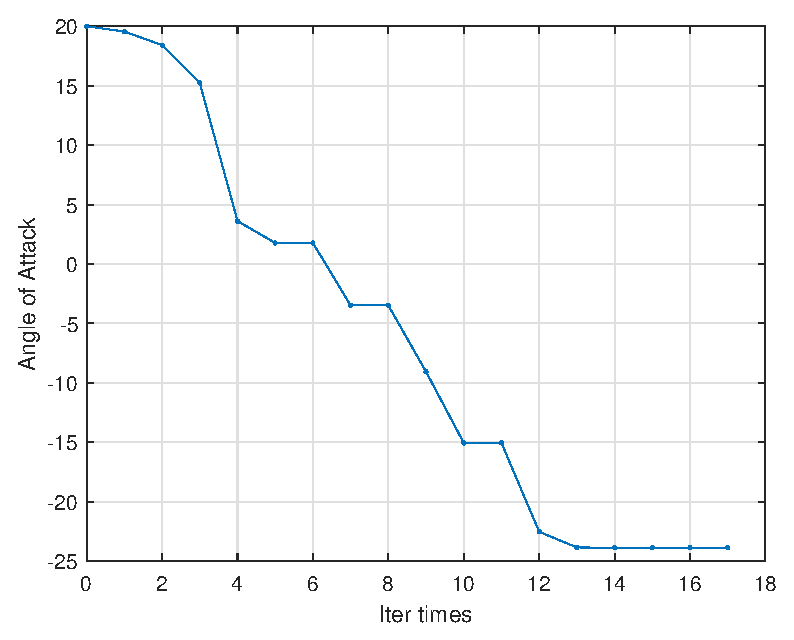
\includegraphics [width=2.9in]{HW3_03.eps}
            \caption{Angle of attack($\alpha$)}
            \vspace{10pt}
    \end{figure}


\newpage
\includepdf[pages=5]{handout.pdf}


\subsection*{Function to plot the iteration state}

\begin{verbatim}
function stop = outputfun(x, optimValue, state)
    stop = false;
    iter_num = optimValue.iteration;

    switch state
        case 'init'
            name = ["Velocity", "Flight Path Angle",
                    "Angle of Attack", "Rate of Climb"];
            for i = 1:3
                figure(i)
                plot(iter_num, x(i), '.-')
                xlabel('Iter times'); ylabel(name(i))
            end
            figure(4)
            plot(iter_num, x(1)*sind(x(3)), '.-')
            xlabel('Iter times'); ylabel(name(4))

        case 'iter'
            if (iter_num ~= 0)
                xdata = 0:iter_num;
                for i = 1:3
                    V_plot = figure(i).Children;
                    V_plot = V_plot.Children;
                    set(V_plot, 'XData', xdata,
                                'YData', [V_plot.YData x(i)])
                end
                V_plot = figure(4).Children;
                V_plot = V_plot.Children;
                set(V_plot, 'XData', xdata,
                            'YData', [V_plot.YData x(1)*sind(x(3))])
            end

        case 'done'
            for i = 1:4
                figure(i); grid on
            end
    end
end
\end{verbatim}

\end{document}

